\begin{frame}
  \frametitle{\problemtitle}
  \begin{block}{Problem}
  	Given a game of Amida-kuji, i.e.\ $k$ legs and some horizontal bars which change over time, decide how many horizontal bars you need to remove to connect the $i$th start to the $i$th end.
  \end{block}
  \begin{center}
  	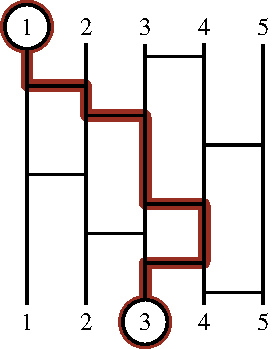
\includegraphics[height=0.65\textheight]{sample}
  \end{center}
\end{frame}

\begin{frame}
	\frametitle{\problemtitle}
	\begin{block}{Solution}
		\begin{itemize}
			\item The game state can be represented by a permutation.
			\item Adding/removing a bar always changes the number of cycles in the permutation by $1$.
			\item We want to build the identity permutation, which has $k$ cycles.
			\pause
			\item There is always a bar whose addition/removal increases the number of cycles.
			\item[$\Rightarrow$] The answer is $k$ minus the number of cycles.			
			\pause
			\item Notice that the actual layout of the bars is irrelevant.
			\item[$\Rightarrow$] We only need to maintain the current permutation (for example with a Segment Tree).
		\end{itemize}
	\end{block}
\end{frame}
